\begin{frame}{Oversampling: where will we see the molecule?}
\underline{Recorded position:} $Y$ is the position of the laser when the molecule is detected;

\[\mathds{P}(Y = y_{r}) = (\mathcal{I}_{\mathds{P}}(t_{0}, \cdot) \star f_{x})(y_{r}) \cdot \prod\limits_{s = 1}^{r - 1} \left(1 - \left(\mathcal{I}_{\mathds{P}}(t_{0}, \cdot) \star f_{X}\right)(y_{s})\right)\]

\begin{figure}[H]
	\label{mapping1}\caption{The sampling design}
	\centering
    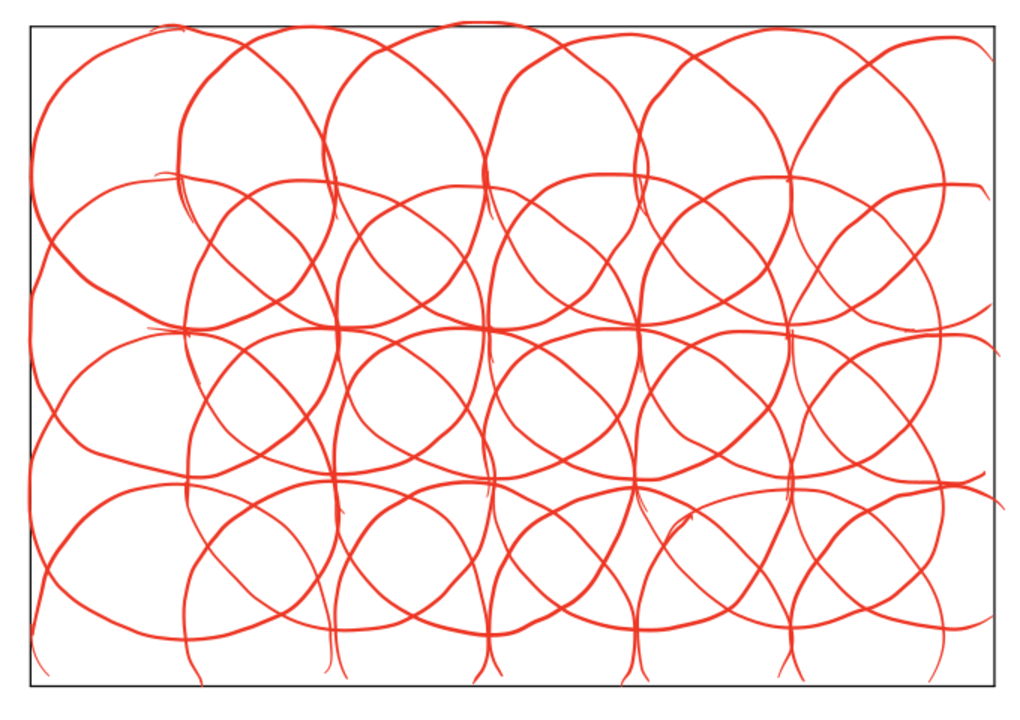
\includegraphics[scale = .3, keepaspectratio]{modelling/oversampling/oversampling.pdf}
\end{figure}

\end{frame}